\documentclass[a4paper,12pt,bibtotocnumbered, twosite]{scrreprt}
\usepackage{caption}
\usepackage{subcaption}
\usepackage{amsmath}
\usepackage{graphicx}
\usepackage{placeins}
\usepackage{float}
\usepackage{array}
\begin{document}

\begin{figure}[h!]
\centering
\begin{subfigure}[l]{0.49\textwidth}
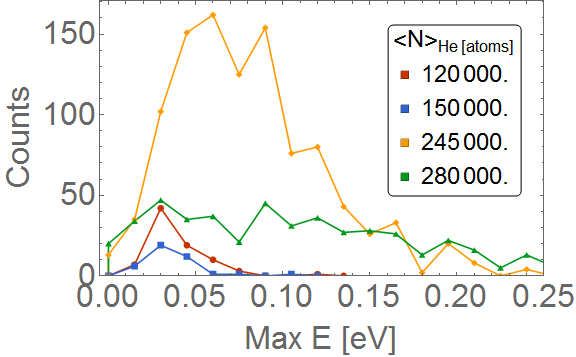
\includegraphics[width=1\textwidth]{../Images/results/Mir_He_Dropletsize/Henerg.png}   				\end{subfigure}
\begin{subfigure}[l]{0.49\textwidth}
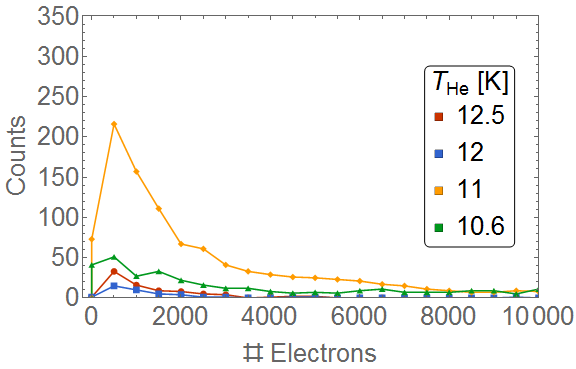
\includegraphics[width=1\textwidth]{../Images/results/Mir_He_Dropletsize/Helec.png} 
\end{subfigure}
\caption[MIR He droplet scan histograms]{On the left, The hitogram for max energy and on rigth, the histogram for number of electrons.}
\label{fig:histodropletsize}
\end{figure}

\end{document}
